\part{Customization}
\begin{frame}
			 \partpage
\end{frame}


\section[Rstudio]{Rstudio Server}
\subsection[rstudiodef]{Defaults and Quirks}
\begin{frame}
  \frametitle{Defaults and Quirks}
	\begin{block}{Defaults}
		\begin{itemize}
			\item Rstudio Server will utilize the default R module unless told otherwise
				\begin{itemize}
					\item Current default is R 4.0.0
				\end{itemize}
			\item Only the dependencies the R module provides are loaded
		\end{itemize}
	\end{block}
	\begin{block}{Quirks}
			\begin{itemize}
			\item The terminal in Rstudio does not start up knowing the modules command
			\begin{itemize}
			\item User can correct this by doing the following commands in the terminal
			\item Changes in this terminals environment (modules loaded/purged) do not change what the R environment sees
			\item . \ctilde{}/.bash\_profile
			\item . /opt/ohpc/admin/lmod/lmod/init/sh
			\end{itemize}
		\end{itemize}
	\end{block}
\end{frame}


\subsection[rstudiodeps]{User defined environment}
\begin{frame}
	\frametitle{Lmod Collections}
	\begin{block}{}
	\begin{itemize}
		\item Lmod has the ability to save/create a named environment (Collections) which can be restored when needed
		\begin{itemize}
			\item For example, a user may create a build environment that loads multiple dependencies and they don't want to load them every single time or remember what they loaded and save it with a name
			\item The user would save the collection by doing "module save build\_enviro" 
			\item The user can then restore the collection by doing "module restore build\_enviro"
		\end{itemize}
		\item  We utilize this mechanism to allow a user to customize their Rstudio environment when using Open OnDemand and allow for the user to:
		\begin{itemize}
			\item Pin the R language version
			\item Load additional dependencies that some of their R libraries require, e.g., netCDF, gdal, CUDA
		\end{itemize}
	\end{itemize}
	\end{block}
\end{frame}


\subsection[rstudioenv]{Requirements \& procedure}
\begin{frame}
	\frametitle{Requirements \& procedure}
	\begin{block}{Requirements}
		\begin{itemize}
			\item The Lmod collection must contain a working R environment
				\begin{itemize}
					\item At a minimum it requires an R module to be loaded - lang/R
				\end{itemize}
			\item The collection must be named "rstudio"
		\end{itemize}
	\end{block}
	\begin{block}{Procedure}
		\begin{enumerate}
			\item Bring up a terminal on the cluster
			\item purge your current module environment
				\begin{itemize}
				\item module purge
				\end{itemize}
			\item Load modules you want to use with R studio
				\begin{itemize}
				\item module load lang/R/3.5.1-intel-2018.5.274-Python-2.7.15 
				\item module load data/GDAL/2.2.3-intel-2018.5.274-Python-2.7.15
				\end{itemize}
			\item Save the module environment to the name "rstudio"
				\begin{itemize}
				\item module save rstudio
				\end{itemize}
			\item Start up a new Rstudio instance and Rstudio should now have the additional libraries and be using the version of R you specified.
		\end{enumerate}
	\end{block}
\end{frame}


\section[Jupyternote]{Jupyter Notebooks}
\subsection[jupenv]{Procedure}
\begin{frame}[fragile]
	\frametitle{Procedure}
	\begin{block}{}
	The following steps were adapted from \url{https://github.com/PSC-PublicHealth/pha-nbextensions}.~\\The following commands should be executed from a compute node in an interactive session prior to starting up a Juypter Notebook in Open OnDemand.
	\end{block}
	\begin{semiverbatim}\footnotesize
	[\$] module load lang/Anaconda3
	[\$] conda create \ddash{}name test\_env python=3
	[\$] source activate test\_env
	\#\#\# Install your required packages \#\#\#
	\# \ldots 
	\# \ldots 
	\#\#\# Finalize setup with these last two packages \#\#\#
	[\$(test\_env)] conda install ipykernel
	[\$(test\_env)] pip install git+https://github.com/PSC-PublicHealth/pha-nbextensions.git
	\#\#\# DONE and ready for use in Open OnDemand \#\#\#
 	\end{semiverbatim}
	\vspace{-1.5em}
	\begin{center}
  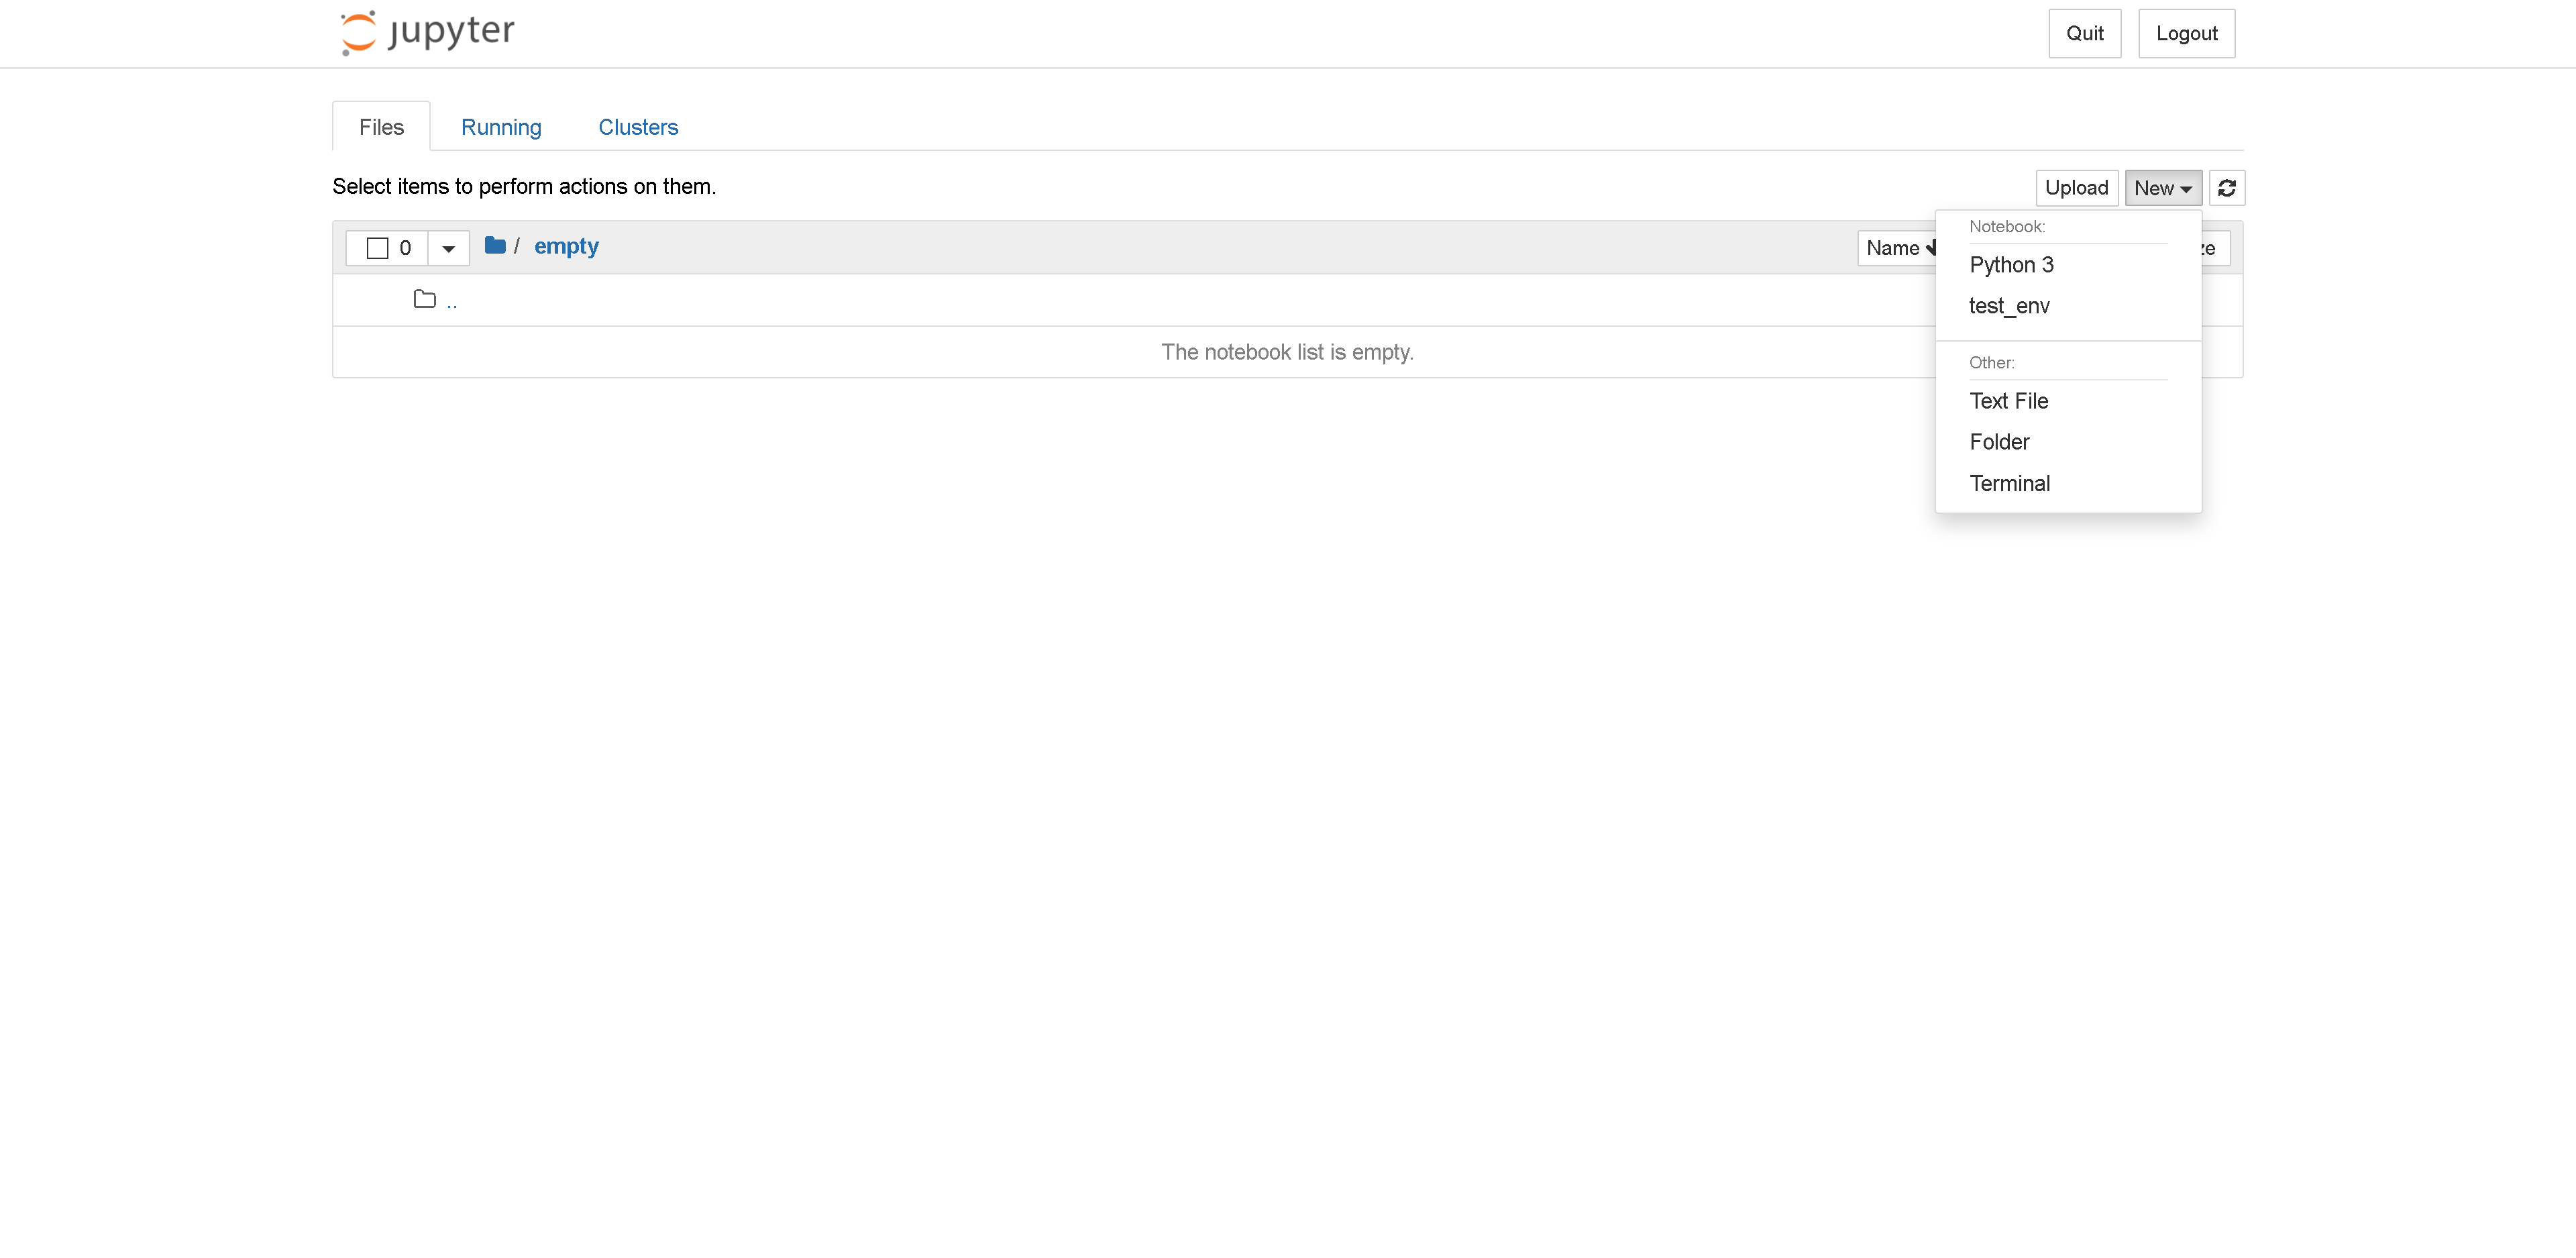
\includegraphics[scale=0.08]{juypter.png}
	\end{center}
	
\end{frame}

